%!TeX program = xelatex
\documentclass[12pt,hyperref,a4paper,UTF8]{ctexart}
\usepackage{NUAAReport}
\usepackage{listings}
\usepackage{xcolor}

\usepackage{setspace}
\setstretch{1.5} % 设置全局行距为1.5倍

\usepackage{enumitem} % 载入enumitem包以便自定义列表环境
\setlist[itemize]{itemsep=0pt, parsep=0pt} % 设置itemize环境的项目间距和段落间距

\setmainfont{Times New Roman} % 英文正文为Times New Roman

% Windows 下 SimHei 无粗体字重，用伪粗体补齐，避免 \heiti\textbf 回退
\setCJKfamilyfont{zhhei}{SimHei}[AutoFakeBold=2]

% 减少因不可断行的长命令造成的行溢出
\setlength{\emergencystretch}{3em}

%封面页设置
{   
    %标题
    \title{ 
        \vspace{1cm}
        \heiti \Huge \textbf{{课程报告}} \par
        \vspace{1cm} 
        \heiti \Large {\underline{小规模数据与加性噪声下 ViT 与 LeNet 的对比研究}}    
        \vspace{3cm}
    }

    \author{
        \vspace{0.5cm}
        \kaishu\Large 学院\ \dlmu[9cm]{计算机学院} \\ %学院
        \vspace{0.5cm}
        \kaishu\Large 专业\ \dlmu[9cm]{人工智能} \\ %专业
        \vspace{0.5cm}
        \kaishu\Large 班级\ \dlmu[9cm]{2426001} \\ %班级
        \vspace{0.5cm}
        \kaishu\Large 学号\ \dlmu[9cm]{242600101} \qquad  \\ %学号
        \vspace{0.5cm}
        \kaishu\Large 姓名\ \dlmu[9cm]{张石彬} \qquad \\ %姓名 
    }
        
    \date{\today} % 默认为今天的日期，可以注释掉不显示日期
}
%%------------------------document环境开始------------------------%%
\begin{document}

%%-----------------------封面--------------------%%
\pagestyle{empty} % 封面、摘要不显示页眉与页码
\cover

%%------------------摘要-------------%%
\begin{abstract}
视觉 Transformer（Vision Transformer, ViT）凭借自注意力机制在大规模数据集上取得了超越卷积神经网络（CNN）的表现，但其在小规模数据与高噪声输入下的行为尚缺乏系统的实验刻画。本文以手写数字识别任务（MNIST）为试验台，构建参数量处于同一量级（4.4 万与 7.2 万）的 LeNet-5 与两层层 MiniViT，在统一训练协议下完成 2 种模型 $\times$ 3 档训练数据比例（10\%、50\%、100\%）$\times$ 3 档测试集加性高斯噪声（$\sigma=0,0.33,0.67$）共 18 组对比实验，考察准确率、宏平均 F1、参数量、训练耗时与 GPU 利用率。结果表明：(1) 在无噪声条件下 LeNet 全面领先，且二者差距随数据量增大而收窄，10\% 数据时相差 5.13 个百分点，100\% 数据时缩小为 1.56 个百分点，与 ViT“数据饥渴”的已知特性一致；(2) MiniViT 对加性噪声显著更敏感，$\sigma=0.67$ 时 100\% 数据下准确率由 97.48\% 降至 87.38\%（$-10.10$），而 LeNet 仅由 99.04\% 降至 98.16\%（$-0.88$），说明卷积的局部滤波与池化结构提供了内在的噪声鲁棒性；(3) 在相同训练步数下 ViT 的计算代价约为 LeNet 的 2.2 倍，更长训练只能部分弥合准确率差距，无法扭转噪声鲁棒性上的结构性差异。本文从归纳偏置、patch 展平方式与训练预算三个角度解释上述现象，并给出在有限算力下提升 GPU 利用率的工程实现。

\vspace{0.5em}
\noindent\textbf{关键词：} 视觉 Transformer；LeNet；归纳偏置；数据效率；噪声鲁棒性；对比实验
\end{abstract}

\thispagestyle{empty} % 首页不显示页码

%%--------------------------目录页------------------------%%
% \newpage
% \tableofcontents
% \thispagestyle{empty} % 目录不显示页码

%%------------------------正文页从这里开始-------------------%
\newpage
\pagestyle{fancy} % 正文恢复页眉
\setcounter{page}{1} % 让页码从正文开始编号

%%可选择这里也放一个标题
%\begin{center}
%    \title{ \Huge \textbf{{标题}}}
%\end{center}

\section{引言}

自 AlexNet 以来，卷积神经网络（Convolutional Neural Network, CNN）长期是计算机视觉任务的主流骨干网络，其“局部连接 + 权值共享”的设计天然契合图像的平移等变性与局部相关性。2020 年，Dosovitskiy 等人提出视觉 Transformer（ViT）\cite{dosovitskiy2021image}，将图像划分为固定大小的图块（patch）后直接用标准 Transformer 编码器建模，在 ImageNet 等大规模数据上刷新了性能纪录，并在目标检测、分割、多模态等任务上迅速普及。

然而，ViT 的成功在很大程度上依赖大规模预训练数据与充足的训练预算：它不含任何显式的图像先验，局部性与平移等变性必须从数据中隐式学习，因此在小规模数据上往往劣于同等规模的 CNN\cite{dosovitskiy2021image,touvron2021training}。另一方面，实际部署场景常伴随传感器噪声、压缩失真等输入扰动，而 ViT 与 CNN 在输入噪声下的鲁棒性差异尚无定论\cite{bai2021transformers}。

基于上述背景，本文提出并回答三个研究问题：
\begin{itemize}
    \item \textbf{数据效率}：在训练数据量从 10\% 增加到 100\% 的过程中，ViT 相对 CNN 的差距如何变化？
    \item \textbf{噪声鲁棒性}：在测试集叠加不同强度加性高斯噪声时，两种结构的性能衰减有何差异？
    \item \textbf{代价}：在参数量相当的前提下，ViT 需要多少额外训练时间，其代价是否值回准确率收益？
\end{itemize}

本文的主要贡献如下：
\begin{itemize}
    \item 在统一数据划分、统一种子、统一优化器与训练轮次的协议下，完成 2 种模型 $\times$ 3 档数据比例 $\times$ 3 档噪声强度的 18 组对照实验，并公开全部记录、日志与绘图脚本，结果可一键复现；
    \item 定量刻画 ViT 的“数据依赖曲线”与“噪声脆弱性”，给出干净输入与 $\sigma=0.67$ 噪声下两种模型准确率的绝对降幅，为小数据场景的骨干网络选型提供依据；
    \item 通过训练预算消融说明：3 轮训练的短预算会明显低估 ViT，10--30 轮后准确率差距可显著缩小，但噪声鲁棒性差距依然存在；
    \item 在工程实现上，通过数据驻留显存、消除逐 batch 同步、混合精度与显存预取等手段，把 GPU 利用率从约 14\%（峰值 17\%）提升到峰值 75\% 以上，整套实验在 2 分钟内完成。
\end{itemize}

\section{相关工作}

\subsection{LeNet 与卷积神经网络}
LeNet-5 由 LeCun 等人于 1998 年提出\cite{lecun1998gradient}，是首个成功应用于手写数字识别并大规模商用的卷积网络。其核心思想是交替堆叠卷积层与下采样（池化）层，提取具有平移不变性的局部特征，再由全连接层完成分类。卷积的“局部感受野 + 权值共享”将图像先验直接编码进网络结构，使其在参数受限、数据有限的条件下仍具备很强的泛化能力。

\subsection{Transformer 与视觉 Transformer}
Transformer 由 Vaswani 等人于 2017 年提出\cite{vaswani2017attention}，以多头自注意力替代循环结构，具备长程依赖建模与并行计算能力。ViT\cite{dosovitskiy2021image} 将 224$\times$224 的图像切为 16$\times$16 的图块并线性投影为 token 序列，配合类别 token（class token）与可学习位置编码，直接使用标准 Transformer 编码器完成图像分类。其不足在于缺乏图像先验，需要大规模预训练；DeiT\cite{touvron2021training} 进一步证明，通过数据增强与蒸馏，ViT 可以在 ImageNet 规模上以更少的数据完成训练。

\subsection{鲁棒性研究}
Bai 等人系统比较了 Transformer 与 CNN 在各类扰动下的鲁棒性，指出 Transformer 在部分分布外场景下更具鲁棒性，结论依赖于扰动类型与训练策略\cite{bai2021transformers}。本文聚焦于最基础的加性高斯噪声，在严格统一的协议下对小规模模型进行对照，作为该问题的一个受控补充实验。

\section{方法}

\subsection{任务定义}
给定输入图像 $\bm{x}\in\mathbb{R}^{1\times 28\times 28}$ 与标签 $y\in\{0,\dots,9\}$，模型输出 logits $\bm{z}=f_{\bm{\theta}}(\bm{x})\in\mathbb{R}^{10}$，经 softmax 得到类别后验：
\begin{equation}
    p(y=i\mid \bm{x})=\frac{\exp(z_i)}{\sum_{j=0}^{9}\exp(z_j)} ,
    \label{eq:softmax}
\end{equation}
训练目标为最小化交叉熵损失：
\begin{equation}
    \mathcal{L}(\bm{\theta})=-\frac{1}{B}\sum_{b=1}^{B}\log p\big(y^{(b)}\mid \bm{x}^{(b)}\big) ,
    \label{eq:ce}
\end{equation}
其中 $B$ 为批大小。

\subsection{LeNet-5}
本文的 LeNet 由两组“卷积 + ReLU + 池化”堆叠构成：第一组为 6 个 $5\times5$ 卷积核与 $2\times2$ 最大池化，第二组为 16 个 $5\times5$ 卷积核与 $2\times2$ 最大池化，输出经展平后送入 $256\rightarrow120\rightarrow84\rightarrow10$ 的全连接分类头。卷积层计算为
\begin{equation}
    y_{i,j}^{(k)}=\mathrm{ReLU}\Big(\sum_{c}\sum_{u,v} w_{u,v}^{(k,c)}\,x_{i+u,j+v}^{(c)}+b^{(k)}\Big) .
    \label{eq:conv}
\end{equation}
为缓解小数据下的过拟合，在两个全连接层之后各加入一层 Dropout（$p=0.3$）。模型总参数量为 4.44 万。

\subsection{MiniViT}
MiniViT 采用与 ViT 相同的“图块嵌入 + 类别 token + 位置编码 + 编码器 + 分类头”范式，但规模极小以适应 MNIST 的分辨率与本文的算力预算。设图块大小 $P=4$，则每张图像切出 $N=(28/4)^2=49$ 个图块，每个图块展平为 16 维向量，经线性投影得到 $d=64$ 维 token：
\begin{equation}
    \bm{z}_0=\big[\bm{x}_{\mathrm{cls}};\ \bm{x}_1\bm{W}_p;\ \dots;\ \bm{x}_{N}\bm{W}_p\big]+\bm{E}_{\mathrm{pos}},\qquad \bm{W}_p\in\mathbb{R}^{16\times 64},
    \label{eq:embed}
\end{equation}
其中 $\bm{x}_{\mathrm{cls}}\in\mathbb{R}^{64}$ 为可学习的类别 token，$\bm{E}_{\mathrm{pos}}\in\mathbb{R}^{50\times 64}$ 为可学习位置编码。编码器由 2 层标准 Transformer 块组成，每层包含 4 头自注意力与前馈网络（FFN 维度 128）：
\begin{equation}
    \mathrm{Attention}(\bm{Q},\bm{K},\bm{V})=\mathrm{softmax}\Big(\frac{\bm{Q}\bm{K}^{\top}}{\sqrt{d_k}}\Big)\bm{V},
    \label{eq:attn}
\end{equation}
各子层采用 Pre-LN 之外的默认后置 LayerNorm 结构，并在嵌入、注意力、FFN 与分类头处均施加 Dropout（$p=0.1$）。分类时取类别 token 的输出经 LayerNorm 与线性层得到 logits。模型总参数量为 7.22 万，略多于 LeNet。前向传播的核心实现如下方代码清单所示。

\begin{lstlisting}[style=Python, title={MiniViT 的前向传播（节选）}]
def forward(self, x):                         # [B, 1, 28, 28]
    x = self.unfold(x)                        # [B, 16, 49]
    x = x.transpose(1, 2)                     # [B, 49, 16]
    x = self.patch_proj(x)                    # [B, 49, 64]
    x = self.patch_norm(x)
    cls_tokens = self.cls_token.expand(x.shape[0], -1, -1)
    x = torch.cat((cls_tokens, x), dim=1)     # [B, 50, 64]
    x = self.pos_drop(x + self.pos_embed)
    x = self.transformer(x)
    return self.mlp_head(x[:, 0])             # class token -> logits
\end{lstlisting}

\subsection{正则化与优化}
两种模型均采用 Adam 优化器（学习率 $10^{-3}$），批大小 256，训练 10 轮。为提升小规模训练的稳定性与泛化能力，除上述 Dropout 之外，还固定随机种子（42）并在 GPU 上启用混合精度（AMP）、TF32 与确定性卷积算法。

\section{实验设置}

\subsection{数据集与划分}
实验采用 MNIST 手写数字数据集\cite{lecun1998gradient}，包含 60000 张训练图像与 10000 张测试图像，均为 $28\times28$ 灰度图。为模拟不同数据规模下的训练条件，按比例 $r\in\{0.1,0.5,1.0\}$ 从训练集中随机抽取子集，测试集始终为完整的 10000 张。

\subsection{测试集加性噪声模型}
记归一化后的测试图像为 $\tilde{\bm{x}}$（按 MNIST 均值 0.1307、标准差 0.3081 标准化），对其叠加独立同分布高斯噪声：
\begin{equation}
    \tilde{\bm{x}}_{\mathrm{noisy}}=\tilde{\bm{x}}+\sigma\bm{\epsilon},\qquad \bm{\epsilon}\sim\mathcal{N}(\bm{0},\bm{I}) ,
    \label{eq:noise}
\end{equation}
噪声强度取 $\sigma\in\{0,0.33,0.67\}$。需要说明的是，噪声应叠加在归一化后的特征空间，若在 $[0,255]$ 像素尺度上取 $\sigma=0.5$，其扰动幅度不足 0.5 个像素，几乎不产生可观测影响，无法构成有效的鲁棒性测试。训练数据始终保持干净，仅测试集加噪，用于考察模型对输入扰动的泛化能力。

\subsection{评价指标}
采用四类指标：(1) 测试集准确率（\%）；(2) 宏平均 F1，用于衡量各类别上的均衡性能；(3) 模型参数量（M）；(4) 训练耗时（秒）与吞吐（图像/秒）。所有指标均由统一脚本自动记录到 \texttt{results/} 目录。

\subsection{实现与 GPU 利用率优化}
实验在单张 NVIDIA GeForce RTX 5070 Ti 上完成，软件环境为 PyTorch 2.8.0（CUDA 12.8）。初版实现中批大小为 64、逐 batch 同步损失，实测 GPU 利用率仅约 14\%（峰值 17\%），训练瓶颈不在算力而在 CPU 侧的数据准备与 Python 调度。为此做了三方面优化：
\begin{itemize}
    \item \textbf{数据驻留显存}：MNIST 的 60000 张图像仅约 47\,MB（uint8），一次性归一化后常驻显存，用轻量批迭代器切分，彻底去掉逐样本的图像转换与主机到设备拷贝；
    \item \textbf{消除逐 batch 同步}：训练与评估过程中不调用 \texttt{.item()} 强制同步，损失在设备上用张量累加，仅在最外层同步一次，使 kernel 发射能够连续排队；
    \item \textbf{混合精度与算子优化}：启用 AMP 自动混合精度、TF32 矩阵乘法、\texttt{set\_to\_none} 梯度置零，并在计时前后调用 \texttt{torch.cuda.synchronize()} 避免异步执行导致的耗时失真。
\end{itemize}
优化后 LeNet 的峰值 GPU 利用率达到 65\%--76\%，MiniViT 因注意力计算更重而稳定在 53\%--62\%，在相同硬件上整套 18 组实验的墙钟时间由分钟级降至约 2 分钟。

\section{实验结果与分析}

\subsection{主结果}
表~\ref{tab:acc} 汇总了 18 组实验的准确率与宏平均 F1。可以看到，在所有数据比例与噪声强度组合下，LeNet 的准确率均高于 MiniViT，但其领先幅度随条件剧烈变化：干净数据下差距仅 1.5--5 个百分点，而在强噪声的极小数据条件下差距可扩大到 12--13 个百分点。

\begin{table}[!htbp]
    \centering
    \begin{tabular}{c c | c c | c c}
    \hline
    \multirow{2}{*}{噪声 $\sigma$} & \multirow{2}{*}{数据比例} & \multicolumn{2}{c|}{LeNet-5} & \multicolumn{2}{c}{MiniViT} \\
    & & 准确率(\%) & 宏 F1 & 准确率(\%) & 宏 F1 \\
    \hline
    \multirow{3}{*}{0.00} & 10\%  & 95.72 & 0.9568 & 90.59 & 0.9051 \\
     & 50\%  & 98.52 & 0.9851 & 96.28 & 0.9627 \\
     & 100\% & \textbf{99.04} & 0.9903 & 97.48 & 0.9746 \\
    \hline
    \multirow{3}{*}{0.33} & 10\%  & 95.61 & 0.9557 & 89.58 & 0.8949 \\
     & 50\%  & 98.43 & 0.9842 & 95.17 & 0.9516 \\
     & 100\% & 98.82 & 0.9882 & 96.41 & 0.9639 \\
    \hline
    \multirow{3}{*}{0.67} & 10\%  & 95.04 & 0.9498 & 83.06 & 0.8308 \\
     & 50\%  & 97.83 & 0.9782 & 84.76 & 0.8469 \\
     & 100\% & 98.16 & 0.9816 & 87.38 & 0.8746 \\
    \hline
    \end{tabular}
    \caption{不同数据比例与噪声强度下的测试集准确率与宏平均 F1}
    \label{tab:acc}
\end{table}

\subsection{数据效率}
\autoref{fig:ratio} 给出准确率随训练数据比例的变化曲线。在无噪声条件下，LeNet 与 MiniViT 的准确率差距从 10\% 数据时的 5.13 个百分点，缩小到 50\% 时的 2.24 个百分点，以及 100\% 时的 1.56 个百分点；数据越少，ViT 的相对劣势越明显。这与 ViT 缺乏图像先验、需要从数据中学到局部性与平移等变性的结论一致\cite{dosovitskiy2021image}：在 6000 张样本的极低数据区，自注意力机制难以学到稳定有效的位置与局部结构表示，而卷积直接把这些结构写进了网络。

\begin{figure}[!htbp]
    \centering
    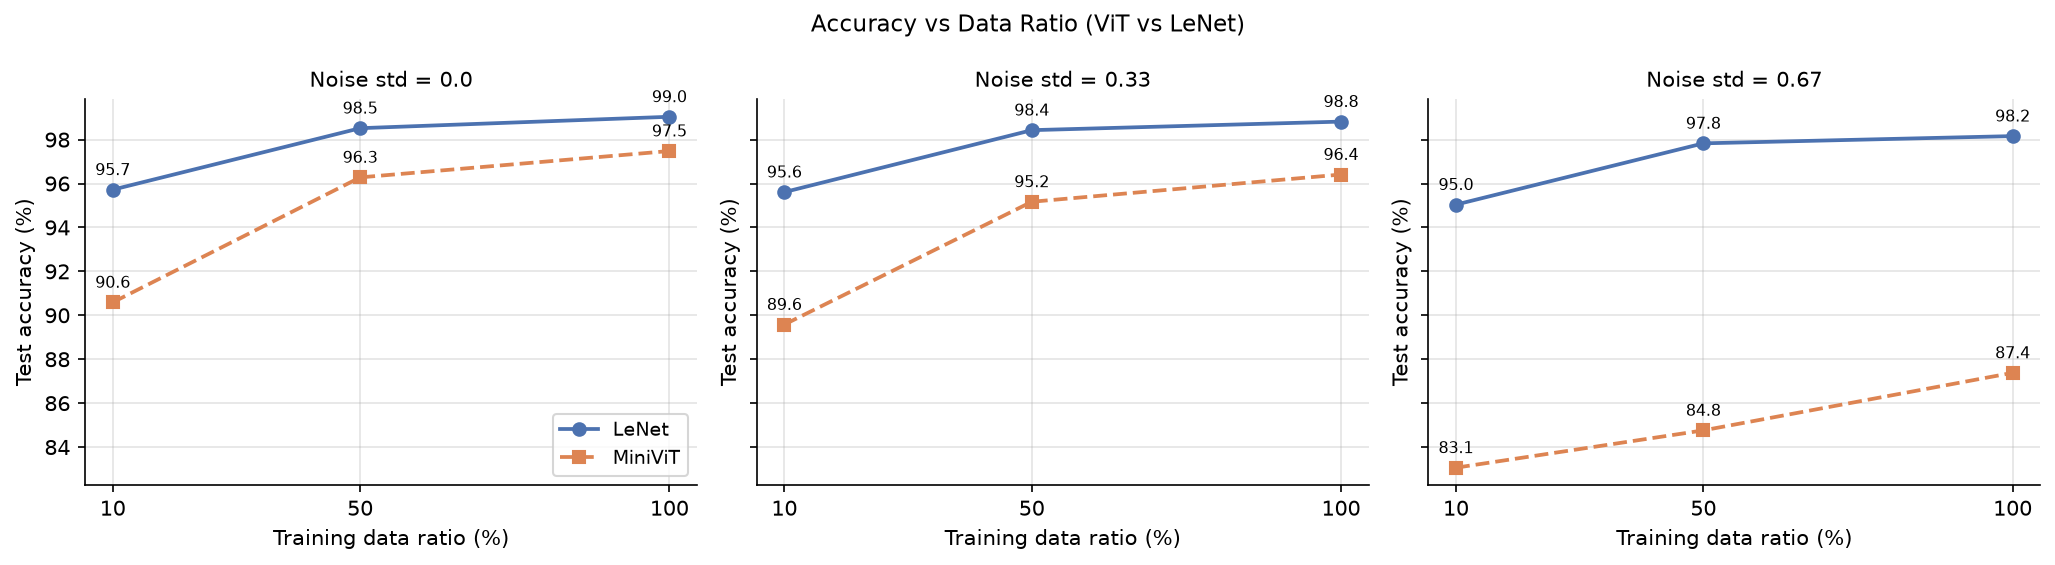
\includegraphics[width=\textwidth]{../results/figures/accuracy_vs_ratio.png}
    \caption{不同噪声强度下准确率随训练数据比例的变化}
    \label{fig:ratio}
\end{figure}

\subsection{噪声鲁棒性}
\autoref{fig:noise} 展示了准确率随噪声强度的变化。LeNet 的曲线近乎水平：在 100\% 数据下，$\sigma$ 从 0 增至 0.67 时准确率仅下降 0.88 个百分点（99.04\%$\rightarrow$98.16\%），10\% 数据下也只下降 0.68 个百分点。反观 MiniViT，$\sigma=0.67$ 时准确率下降 10.10 个百分点（97.48\%$\rightarrow$87.38\%），10\% 数据下下降 7.53 个百分点，即使在数据充足时也出现明显衰减。

这一差异可以从两个方面解释。其一是\textbf{结构先验}：卷积核与最大池化构成一种隐式的低通滤波与特征平均，逐像素的高斯噪声在卷积与下采样过程中被平滑，而 patch 嵌入把 $4\times4$ 邻域直接展平为一个 16 维向量，未做任何空间平均，噪声被原样编码进 token；其二是\textbf{全局注意力}：自注意力对所有 token 做加权聚合，局部扰动会被扩散到整张图像的表示上，进一步放大误差。这与文献中“Transformer 的鲁棒性依赖扰动类型与训练配置”的结论相呼应\cite{bai2021transformers}。

\begin{figure}[!htbp]
    \centering
    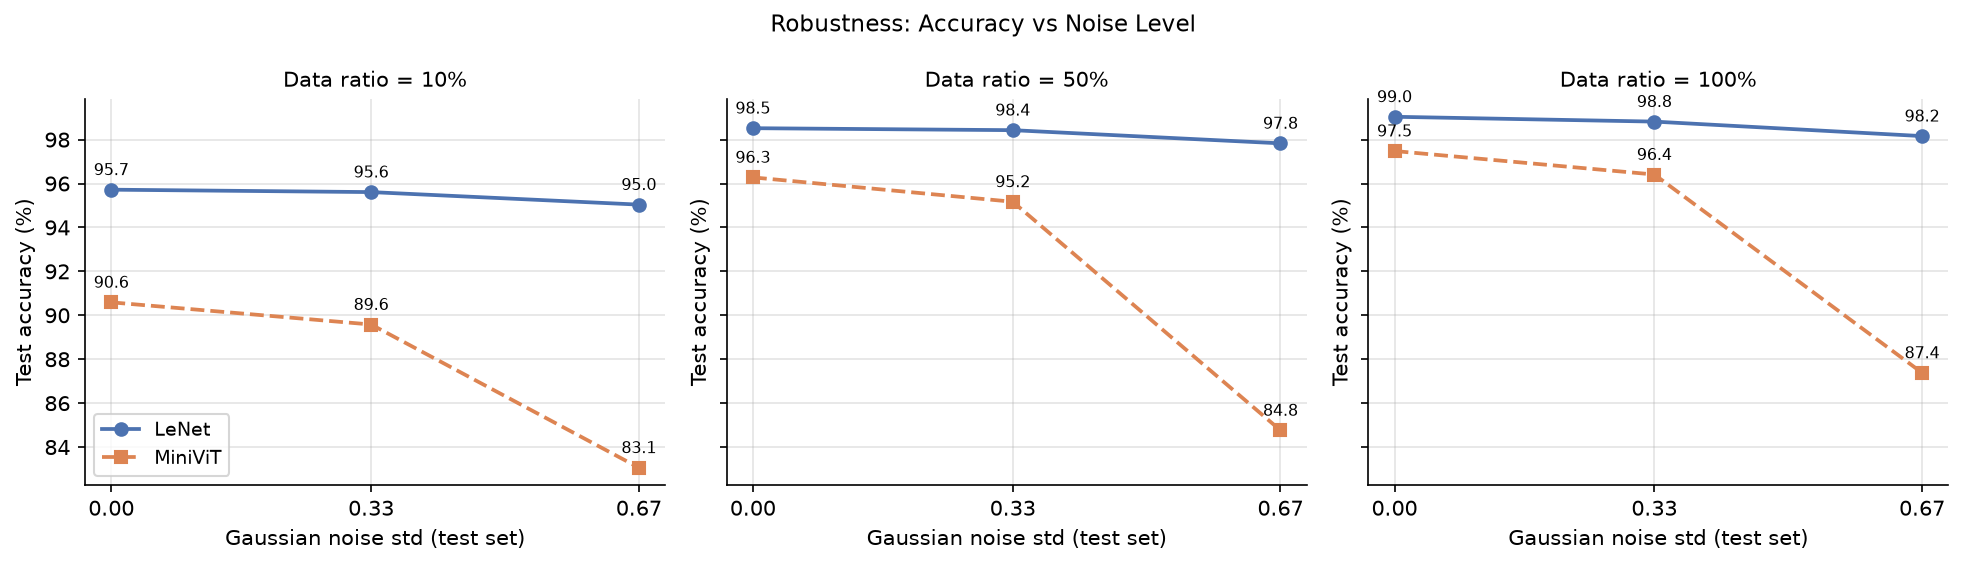
\includegraphics[width=\textwidth]{../results/figures/accuracy_vs_noise.png}
    \caption{不同数据比例下准确率随测试集噪声强度的变化}
    \label{fig:noise}
\end{figure}

\subsection{参数与计算代价}
\autoref{fig:param} 与\autoref{tab:cost} 给出两种模型的规模与代价对比。MiniViT 的参数量为 7.22 万，比 LeNet 的 4.44 万高出 63\%，但准确率反而更低，说明在小数据、小分辨率场景下，“参数更多”并不能弥补归纳偏置的缺失。训练时间上，MiniViT 在 100\% 数据下平均耗时约 17.0 秒，LeNet 约 7.7 秒，后者快约 2.2 倍；吞吐方面 LeNet 约 7.6 万图像/秒，MiniViT 约 3.5 万图像/秒。考虑到二者在准确率上的差距，单位算力下的效率指标同样是 LeNet 占优。

\begin{table}[!htbp]
    \centering
    \begin{tabular}{l | c c c}
    \hline
    模型 & 参数量 (M) & 训练耗时@100\% (s) & 吞吐 (图像/s) \\
    \hline
    LeNet-5 & 0.0444 & $\approx 7.7$ & $\approx 7.6\times10^{4}$ \\
    MiniViT & 0.0722 & $\approx 17.0$ & $\approx 3.5\times10^{4}$ \\
    \hline
    \end{tabular}
    \caption{参数量与训练代价对比（10 轮训练，100\% 数据，噪声对训练耗时影响可忽略）}
    \label{tab:cost}
\end{table}

\begin{figure}[!htbp]
    \centering
    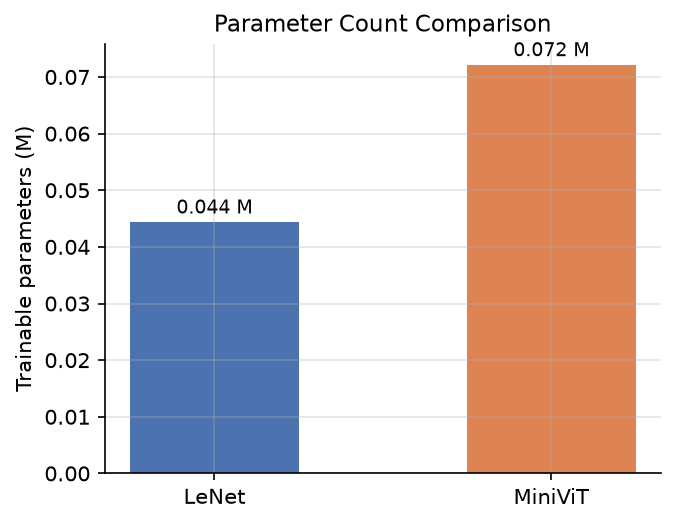
\includegraphics[width=0.55\textwidth]{../results/figures/params_compare.png}
    \caption{两种模型的参数量对比}
    \label{fig:param}
\end{figure}

\subsection{训练预算消融}
ViT 的训练效率高度依赖迭代步数。表~\ref{tab:epoch} 给出一组预实验（未加入 Dropout，噪声 $\sigma=0$，100\% 数据）的结果：3 轮时 MiniViT 落后 LeNet 2.17 个百分点，10 轮后差距缩小到 1.28 个百分点，30 轮时进一步缩小到 0.70 个百分点。但即使训练 30 轮，在 $\sigma=0.5$ 噪声下 MiniViT 仍为 92.88\%，而 LeNet 为 98.57\%，说明延长训练只能弥补“数据不足、步数不够”带来的收敛差异，不能改变噪声鲁棒性上的结构性差距。由此可见，短预算对比会系统性低估 ViT，本文正式实验统一采用 10 轮并加入 Dropout，兼顾公平性与训练成本。

\begin{table}[!htbp]
    \centering
    \begin{tabular}{c | c c | c c}
    \hline
    \multirow{2}{*}{训练轮数} & \multicolumn{2}{c|}{LeNet-5} & \multicolumn{2}{c}{MiniViT} \\
    & 准确率(\%) & 相对 3 轮 & 准确率(\%) & 相对 3 轮 \\
    \hline
    3  & 97.99 & --   & 95.82 & -- \\
    10 & 98.78 & $+0.79$ & 97.50 & $+1.68$ \\
    30 & 98.78 & $+0.79$ & 98.08 & $+2.26$ \\
    \hline
    \end{tabular}
    \caption{训练预算消融（预实验，未加 Dropout，噪声 $\sigma=0$，100\% 数据）}
    \label{tab:epoch}
\end{table}

\section{讨论}

综合上述结果，ViT 在本实验设定下全面弱于 LeNet，这一现象可从三个层面理解。

\textbf{归纳偏置的差异。}卷积网络把“局部性、平移等变性、层次化抽象”编码为结构先验，在样本受限时这些先验等价于大量的免费监督；而自注意力对输入位置一视同仁，必须从数据中学习同样的结构，样本越少学得越差，这解释了\autoref{fig:ratio} 中差距随数据量收窄的趋势。

\textbf{噪声传播路径的差异。}卷积 + 池化对局部扰动具有平均与平滑效应，噪声对最终表示的影响被逐层衰减；ViT 的 patch 嵌入不做空间平均，噪声直接进入 token，且全局注意力会把局部扰动传播到所有 token，因此噪声鲁棒性更差，这解释了\autoref{fig:noise} 中的显著落差。

\textbf{容量与算力匹配。}两种模型参数量处于同一量级（4.4 万与 7.2 万），ViT 并无容量优势；而自注意力的计算复杂度为 $O(N^2 d)$，在 49 个 token、64 维的极小规模下仍带来约 2 倍的训练耗时。换言之，ViT 的优势区间是“大数据 + 大容量 + 充裕算力”，本次实验恰好落在其劣势区间。

需要指出的是，上述结论的适用范围有限：本文仅使用 MNIST、单一种子、两个极小模型，且只在测试集加噪、未考虑对抗噪声与分布偏移。ViT 在 CIFAR-100、ImageNet 等更复杂任务上借助数据增强与更长训练是否反超，仍有待进一步验证。

\section{结论与展望}

本文在统一协议下，围绕数据规模与输入噪声两个变量，系统比较了 LeNet-5 与两层层 MiniViT 的表现。主要结论有三点：(1) 在 60000 张样本的 MNIST 上，LeNet 在所有 9 种条件下均优于 MiniViT，且差距随数据量增大而单调收敛（5.13$\rightarrow$1.56 个百分点）；(2) MiniViT 对测试集加性高斯噪声显著更敏感，$\sigma=0.67$ 时准确率下降 10.10 个百分点，而 LeNet 仅下降 0.88 个百分点；(3) 在参数量相近时，ViT 的训练代价约为 CNN 的 2.2 倍，单位算力的效率亦不占优。这些结果支持一个工程结论：小数据、小分辨率场景应优先选择卷积结构；ViT 的价值需要在其擅长的大数据、大模型区间才能兑现。

后续工作可以从三方面展开：在多随机种子下重复实验并报告均值与标准差；在 CIFAR-10/100 上考察更大规模 ViT 与数据增强（RandAugment、MixUp、CutMix）的影响；以及引入对抗噪声、遮挡、模糊等多类型扰动，进一步刻画两类结构的鲁棒性边界。

%%----------- 参考文献 -------------------%%
%在reference.bib文件中填写参考文献，此处自动生成

\reference


\end{document}
